%=============================================================================
% Thesis Template in LaTex
%
% File:  06-Diskussion.tex -- Diskussion
% Author(s): Cyrano Golliez <golliezc@student.ethz.ch>
%
% Creation:  27 Jan 2014
% Time-stamp: <Tue 2013-08-13 20:14 juergen>
%
% Copyright (c) 2014 Infrastructure Management Group (IMG)
%               http://ibi.ethz.ch
%
% More information on LaTeX: http://www.latex-project.org/
%=============================================================================

\chapter{Diskussion}
\label{chap:Diskussion}

In diesem Kapitel wird die in Abschnitt \ref{chap:Resultate} als optimal erachtete Lösung untersucht. Einerseits werden die Zustände 1 bis 4 mit dem Grundzustand 0 verglichen und andererseits die einzelne Kostenstrukturen in den verschiedenen Zuständen untersucht. Dies geschieht, um die als optimal erachtete Variante auf ihre Belastbarkeit in einer allfälligen Diskussion zuprüfen.

\paragraph{Zustand 0}

Gemäss dem Risikovergleich in Abschnitt \ref{chap:Resultate} ist im Zustand 0 die bestmögliche Variante für die Zukunft von Uster die Variante 2.  
Bei näherer Betrachtung der in Abbildung \ref{img:KostenZ0} dargestellten Reisezeitkosten und Unterhaltskosten der Varianten wird verdeutlicht, dass die Kosten die in der Variante 1 aufgrund der verlängerten Wartezeit entstehen, die Mehrkosten infolge Bau und Wartung der Variante 2, bei einer Betrachtung der Gesamtkosten über einen Zeitraum von 40 Jahren, um ein vielfaches übersteigen. Die Mehrkosten die bei der Ausführung der Variante 2 infolge höherer Bau- und Wartungskosten enstehen, betragen 1'238'600 CHF wohingegen die Mehrkosten die infolge der Variante 1, aufgrund der höheren Reisezeitkosten entstehen 38'984'439 CHF betragen. 

Durch diesen Vergleich wird verdeutlicht, dass sich die Variante 1, welche die Option "nichts zu verändern" darstellt, über den betrachteten Zeitraum von 40 Jahren nicht lohnenen wird. Die Mehrkosten die den Nutzern des Bahnübergangs und somit auch indirekt der Stadt Uster infolge der verlängerten Wartezeit entstehen, übersteigen die geforderten Inverstitionskosten für den Bau der Velounterführung um ein vielfaches. Im Fall der Variante 3 trifft dies nicht zu, weshalb sich ein solches Inverstment unter den Annahmen des Grundzustandes nicht lohnt.

\begin{figure}[h!]
  \centering
  \subfloat[][]{\label{img:}\includegraphics[width=.45\textwidth]{./figures/06-01-Unterhaltskosten-Z0}}
  \hfill
  \subfloat[][]{\label{img:}\includegraphics[width=.45\textwidth]{./figures/06-02-Reisezeitkosten-Z0}}
\caption[Verkehrsaufkommen]{Tägliches Verkehraufkommen Brunnenstrasse}
  \label{img:KostenZ0}
\end{figure}

\begin{IMleftrightskip}
Die Kosten wurden analog der in Abschnitt \ref{subsec:BerechnungRisiken} erläuterten Risikoberechnung ermittelt. Dies gilt für alle weiteren erwähnten Kostenstrukturen.
\end{IMleftrightskip}

Demnach lohnt sich der Bau der Variante 2 für die Stadt Uster bei einer Betrachtung der Gesamtkosten über 40 Jahre und das entstehende Risiko rechtfertigt die höheren Investitionskosten zu Beginn des untersuchten Zeitraum. 

\paragraph{Zustand 1}

Gemäss Abschnitt \ref{chap:Resultate} ist auch in Zustand 1 die Variante 2 die optimale Lösung. Somit hat die Veränderung des E-Auto Anteiles keinen Einfluss auf die Wahl der optimalen Variante. \\
Infolge des Vergleichs der Zustände 0 und 1 ist ersichtlich, dass das Risiko der Variante 1 um 0.023\%, das Risiko der Varianten 2 um 0.024\% und das Risiko der Variante 3 um 0.017\% gegenüber dem jeweiligen Risiko im Zustand 0 ansteigt. Diese Abweichungen wäre, um den Effekt der die Veränderung des E-Auto Anteiles auf optimale Lösung hat, im Rahmen einer Hauptstudie zu untersuchen.

Bei der näheren Betrachtung der Umweltkosten wird ersichtlich, dass die Umweltkosten für alle 3 Varianten jeweils um einen Betrag von 163'555 CHF ansteigen. 
Ein konservative Prognose des E-Auto Anteil hat somit keinen Einfluss auf die Wahl der optimalen Variante. Demnach müsste die Variante 2 auch in einer Zukunft in der der Verbrennungsmotor weiterhin eine massgebende Rolle spielen wird, die als optimal zu erachtetende Variante sein, um die Verkehrssituation am Bahnübergang nachhaltig zu verbessern.


\paragraph{Zustand 2} 

Wie im Abschnitt \ref{chap:Resultate} dargestellt, hat die Veränderung der Unfallwahrscheinlichkeit keinen Einfluss auf die Wahl der optimalen Variante. 
Bei näherer Betrachtung der Unfallkosten, sieht man, dass sich die Veränderung der Unfallwahrscheinlichkeit deutlich auf die anfallenden Unfallkosten auswirkt. 
Die Abbildung \ref{img:UnfallVer.Z0-2} zeigt den Unfallkostenvergleich der Zustände 0 und 2. Die Unfallkosten aller Varianten im Zustand 0 betragen 451'469 CHF. Im Zustand 2 betragen die Unfallkosten der Variante 2 547'384 CHF und die Unfallkosten der Variante 3 321'649 CHF. Für die Variante 2 entspricht das einer Veränderung von 21.25\% und für die Variante 3 einer Abnahme von 28.75\%. 

\begin{figure}[h!]
	\centering
	\includegraphics[width=.45\textwidth]{figures/06-03-Unfallkostenvergleich-Z0-Z2}
	\caption[Unfallkostenvergleich: Zustand 0 und 2]{Unfallkostenvergleich: Zustand 0 und 2}
	\label{img:UnfallVer.Z0-2}
\end{figure}

Betrachtet nun hingegen die Veränderung der Risiken der Variante von Zustand 0 zu Zustand 2, so beträgt die Veränderung für die Variante 1 +0.01\% und für die Variante 3 -0.01\%. 
Somit ist die Variante 2 auch mit erhöhter Unfallgefahr die optimale Variante für die zukünftige Situation am Bahnübergang Brunnenstrasse. 
 

\paragraph{Zustand 3} 

Die Veränderung der Eintrittswahrscheinlichkeit, wie in Abschnitt \ref{subsec:Sensitivitätsanalyse} dargestellt, hat keinen Einfluss auf die Wahl der optimalen Variante. Jedoch ist die folgende Darstellung \ref{img:SzeVer-Z0} der Risiken der einzelnen Szenarien, insofern interessant, dass es den Effekt verdeutlicht der die Wahl der Eintrittswahrscheinlichkeit auf die Verteilung der Risiken hat. So kann mit der Gewichtung der möglichen zukünftigen Ereignisse, sprich den Prognosen der möglichen Zukunft, die berechneten Risiken beeinflusst werden. 

\begin{figure}[h!]
	\centering
	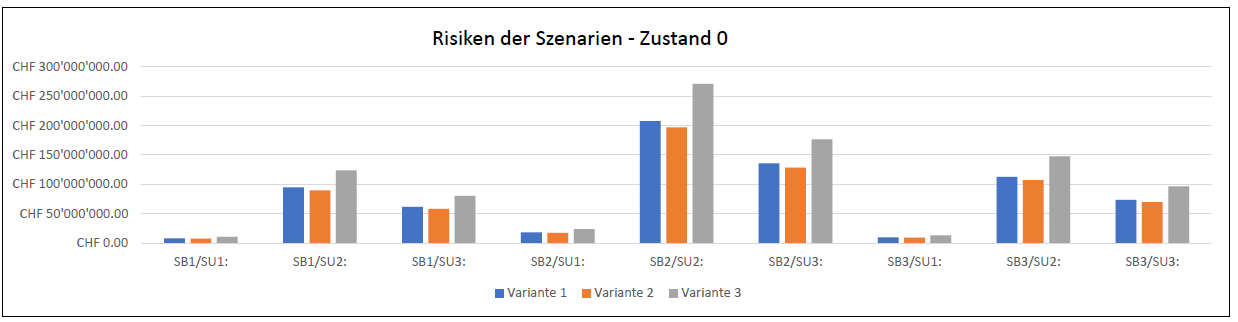
\includegraphics[width=.45\textwidth]{figures/f-06-04-RisikenSzenarienZ0}
	\caption[Szenarienvergleich im Zustand 0]{Vergleich der Risiken der Szenarien im Zustand 0}
	\label{img:SzeVer-Z0}
\end{figure} 

Im Zustand 3 wird der Schwerpunkt der Gewichtung der Szenarien so gelegt, dass diejenigen Szenarien mehr gewicht erhalten, welche die höchsten Wachstumsprognosen voraussagen und demnach das grösste Verkehrsaufkommen simulieren. Der Effekt einer solchen Verschiebung auf die Szenarien wird in der nachfolgenden Abbildung \ref{img:SzeVer-Z3} verdeutlicht. 

\begin{figure}[h!]
	\centering
	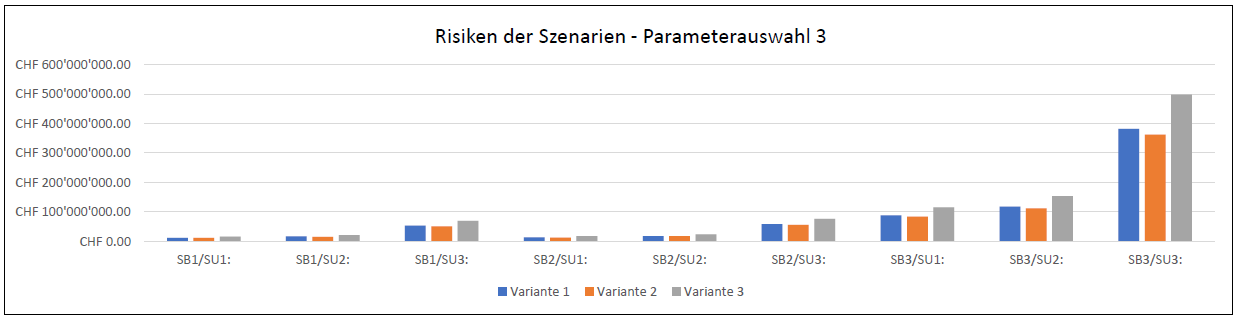
\includegraphics[width=.45\textwidth]{figures/f-06-05-RisikenSzenarienZ3}
	\caption[Szenarienvergleich im Zustand 3]{Vergleich der Risiken der Szenarien im Zustand 3}
	\label{img:SzeVer-Z3}
\end{figure} 

Auf die Wahl der optimalen Variante hat diese Veränderung keinen Einfluss, da die Risiken der Varianten jeweils um 5.5\% im Vergleich zum Zustand 0 steigen. Erst bei der Betrachtung der Nachkommastellen, lässt sich eine gewisse Unterscheidung feststellen. So beträgt die Veränderung des Risiko der Variante 1 vom Zustand 0 zum Zustand 3 5.530\%, die Veränderung des Risiko der Variante 2 beträgt 5.518\% und die Veränderung des Risikos der Variante 3 5.525\%. Aus diesen geringfügigen Abweichung einen Rückschluss auf die im Rahmen des Zustand 3 veränderten Eigenschaften der Risikoberechnung zu machen, war im Rahmen dieser Projektarbeit nicht möglich und wäre im Rahmen einer Hauptstudie weiter zu untersuchen.


\paragraph{Zustand 4} 

Wie in Abschnitt \ref{chap:Resultate} ermittelt, ist im Zustand 4 das Risiko der Variante 3 um 38'095 CHF kleiner als das Risiko der Variante 2. Das Risiko der Variante 1 bleibt unverändert und aufgrund dessen ist die optimale Variante im Zustand 4 die Variante 3. \\
Die getroffenene Annahme über die Wartezeit der Variante 3 in Zustand 4 vernachlässigt das Ampelsystem und berücksichtigt demnach nicht, eine verlängerte Reisezeit aufgrund der Rotlichtzyklen des Ampelsystems. 

Den Einfluss dieser Veränderund sieht man verdeutlicht bei der näheren Betrachtung der Reisezeitkosten. So nehmen die Reisezeitkosten der Variante 3 von Zustand 0 zu Zustand 4 um  257'694'277 CHF ab, wie in Abbildung \ref{img:ReisezeitkostenZ0-Z4} ersichtlich ist. Die Reisezeitkosten der Varianten 1 und 2 bleiben im Zustand 4 unverändert, da ihre gemäss Abschnitt \ref{sec:Kostenstruktur} definierten Parameter der Kostenberechnung nicht verändert werden. So betragen die Reisezeitkostend der Variante 1 sowohl in Zustand 0 als auch in Zustand 4 705'874'810 CHF und die Reisezeitkosten der Variante 2 666'890'370 CHF.


\begin{figure}[h!]
	\centering
	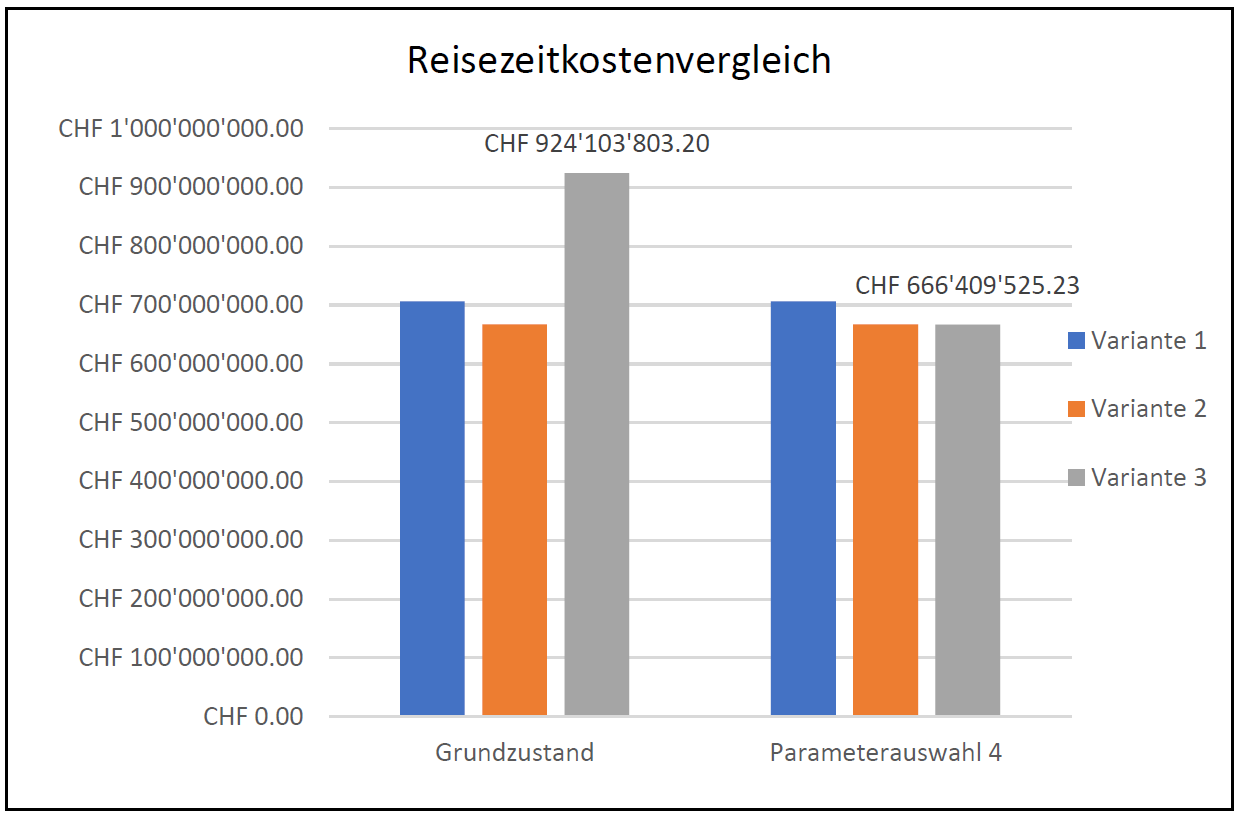
\includegraphics[width=.45\textwidth]{figures/f-06-06-ReisezeitVergleichZ0-Z4}
	\caption[Reisezeitkostenvergleich Zustand 0 und 4]{Vergleich der Reisezeitkosten der Zustände 0 und 4}
	\label{img:ReisezeitkostenZ0-Z4}
\end{figure} 

Bei näherer Betrachtung der Reisezeitkosten der Variante 2 und Variante 3 wird verdeutlicht wieso die Variante 3 im Zustand 4 das gerinste Risiko generiert. \\
In Abbildung \ref{img:ReisezeitkostenV2-V3-Z4} ist ersichtlich, dass die Reisezeitkosten der Variante 2 ... CHF betragen und die Reisezeitkosten der Variante 3 in Zustand 4 nur noch .... CHF. So nehmen die Reisezeitkosten der Variante 3 in Zustand 4 um 27.89\% gegenüber Zustand 0 ab. Das Risiko hingegen der Variante 3 im Zustand 4 nimmt um 27.38\% gegenüber dem Risiko in Zustand 3 ab.

\begin{figure}[h!]
	\centering
	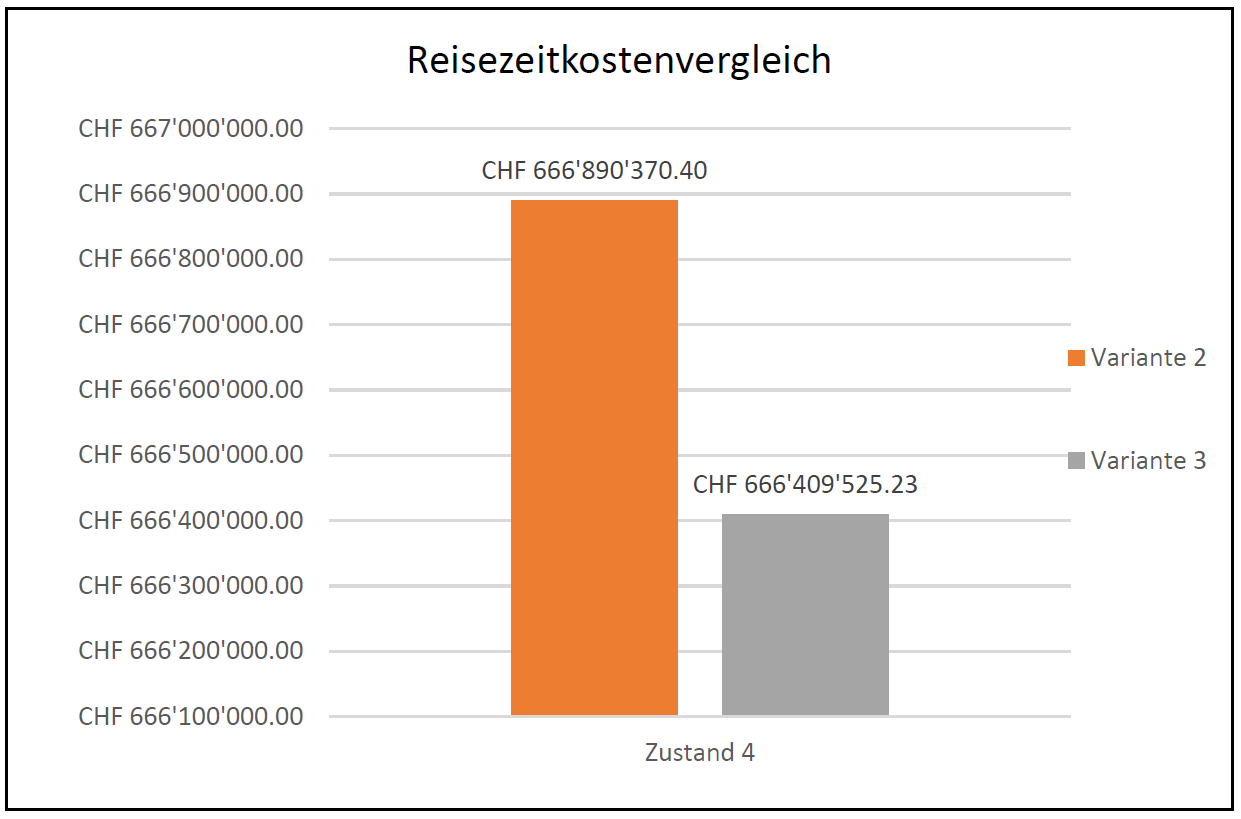
\includegraphics[width=.45\textwidth]{figures/f-06-07-ReisezeitVergleichV2_V3-Z0}
	\caption[Reisezeitkostenvergleich Variante 2 und 3 in Zustand 4]{Vergleich der Reisezeitkosten der Varianten 2 und 3 im Zustand 4}
	\label{img:ReisezeitkostenV2-V3-Z4}
\end{figure} 

Die Differenz der Reisezeitkosten der Varianten 2 und 3 beträgt 480'845 CHF, wobei die Differenz der Risiken der Varianten 2 und 3 im Zustand 4 gemäss Abschnitt \ref{chap:Resultate} 38'095 beträgt. So wird verdeutlicht, dass einerseits die Reisezeit der entscheidende Faktor für der Risikoberechnug ist und andererseits das die im Rahmen der Optimierung des Bahnübergangs Brunnenstrasse notwendigen Entscheidungsprozese, von den Annahmen der zu erwartenden Reisezeiten abhängig ist.
Des weitern ist ersichtlich, dass die Mehrkosten die beim Bau der Variante 3 im Vergleich zu Variante 2 entstehen, gemäss Abschnitt \ref{sec:Varianten} 347'750 CHF, von den grösseren Reisezeitkosten der Variante 2 kompensiert werden. Die verbleibende Differenz der Risiken von 38'095 CHF und die daraus folgende Wahl der Variante 3 als optimale Variante muss, aufgrund dessen das die getroffenen Annahmen des Zustand 4 nicht unbedingt der Wirklichkeit entsprechen, von einem kritischen Standpunkt aus betrachtet werden.

Meiner Meinung nach entspricht die getroffenen Annahme, dass die Wartezeit der Variante 3 aufgrund der Einführung eines Ampelsystem nicht ansteigt, nicht der Wirklichkeit. \\
So wird bei der Betrachtung der jetztigen Situation am Bahnübergang klar, dass sich die Wartezeit aufgrund von Rückstaus, bedingt durch die Verkehrsüberlastung der Innenstadt, zu Hauptverkehrszeiten deutlich verlängert. Infolge wird die Einführung eines Ampelsystems aufgrund der beengten Platzverhältnisse vor Ort zu, wie in den Zuständen 0 bis 3 angenommen, einer erhöhten Wartezeit führen, was den Annahmen des Zustand 4 wiederspricht.

Die Wahl der Variante 3 zur optimalen Variante im Zustand 4 hat infolge der Diskussion der Annahmen, auf den Entscheidungsprozes keine Einfluss.
Nimmt man an, dass sich die Wartezeiten für alle 3 Varianten, aufgrund der Einführung einer neuen S-Bahn Linie gleichmässig erhöht, so lohnt sich meiner Meinung nach das grössere Investment der Variante 3 nur bei einer Betrachtung der Situation über einen Zeitraum von vierig Jahren. Die Variante 3 könnte sich insofern für die Stadt Uster lohnen, da das eingeführte Ampelsystem eine Verschiebung des innerstädtischen Modalsplit zur Folge haben kann und demnach der Veloverkehr gefördert wird, was sich wiederum in den Unfall- und Umweltbelastungskosten wiederspiegelt.

In dieser Diskussion werden die Mehrwerte der Variante 3, die aufgrund der erhöhten Sicherheit sowie des erhöhten Fahrkomfort entstehten, ausser Acht gelassen. 
Dieser Mehrwert, den ich im Rahmen diesere Optimierung nicht modelliert habe, muss, um die Varianten 2 und 3 vertieft vergleichen zu können, ermittelt werde. Die Velounterführung der Variante 2 mit ihren 1.5 Meter lichten Breite hat im Vergleich zur Variante 3 mit über 2 Metern Durchfahrtsbreite, einen deutlich geringeren Fahrkomfort und demtentsprechend in der Realität auch ein erhöhtes Unfallrisiko. Somit kann für den Zustand 4, mit den mir zur Verfügung stehenden Mitteln nicht abschliessend geklärt werden ob die Variante 3 die als optimal zu erachtende Variante ist.
      

% ===========================================================================
% EOF
%

%%% Local Variables:
%%% mode: latex
%%% TeX-master: "../main"
%%% End:
